%
%Не забыть:
%--------------------------------------
%Вставить колонтитулы, поменять название на титульнике



%--------------------------------------

\documentclass[a4paper, 12pt]{article} 

%--------------------------------------
%Russian-specific packages
%--------------------------------------
%\usepackage[warn]{mathtext}
\usepackage[T2A]{fontenc}
\usepackage[utf8]{inputenc}
\usepackage[english,russian]{babel}
\usepackage[intlimits]{amsmath}
\usepackage{esint}
%--------------------------------------
%Hyphenation rules
%--------------------------------------
\usepackage{hyphenat}
\hyphenation{ма-те-ма-ти-ка вос-ста-нав-ли-вать}
%--------------------------------------
%Packages
%--------------------------------------
\usepackage{amsmath}
\usepackage{amssymb}
\usepackage{amsfonts}
\usepackage{amsthm}
\usepackage{latexsym}
\usepackage{mathtools}
\usepackage{etoolbox}%Булевые операторы
\usepackage{extsizes}%Выставление произвольного шрифта в \documentclass
\usepackage{geometry}%Разметка листа
\usepackage{indentfirst}
\usepackage{wrapfig}%Создание обтекаемых текстом объектов
\usepackage{fancyhdr}%Создание колонтитулов
\usepackage{setspace}%Настройка интерлиньяжа
\usepackage{lastpage}%Вывод номера последней страницы в документе, \lastpage
\usepackage{soul}%Изменение параметров начертания
\usepackage{hyperref}%Две строчки с настройкой гиперссылок внутри получаеммого
\usepackage[usenames,dvipsnames,svgnames,table,rgb]{xcolor}% pdf-документа
\usepackage{multicol}%Позволяет писать текст в несколько колонок
\usepackage{cite}%Работа с библиографией
\usepackage{subfigure}% Человеческая вставка нескольких картинок
\usepackage{tikz}%Рисование рисунков
\usepackage{float}% Возможность ставить H в положениях картинки
% Для картинок Моти
\usepackage{misccorr}
\usepackage{lscape}
\usepackage{cmap}
\usetikzlibrary{arrows}
\usepackage{cancel}

% Для Х И М И И

\usepackage[version=4]{mhchem}



\usepackage{graphicx,xcolor}
\graphicspath{{Pictures/}}
\DeclareGraphicsExtensions{.pdf,.png,.jpg}

%----------------------------------------
%Список окружений
%----------------------------------------
\newenvironment {theor}[2]
{\smallskip \par \textbf{#1.} \textit{#2}  \par $\blacktriangleleft$}
{\flushright{$\blacktriangleright$} \medskip \par} %лемма/теорема с доказательством
\newenvironment {proofn}
{\par $\blacktriangleleft$}
{$\blacktriangleright$ \par} %доказательство
%----------------------------------------
%Список команд
%----------------------------------------
\newcommand{\grad}
{\mathop{\mathrm{grad}}\nolimits\,} %градиент

\newcommand{\diver}
{\mathop{\mathrm{div}}\nolimits\,} %дивергенция

\newcommand{\rot}
{\ensuremath{\mathrm{rot}}\,}

\newcommand{\Def}[1]
{\underline{\textbf{#1}}} %определение

\newcommand{\RN}[1]
{\MakeUppercase{\romannumeral #1}} %римские цифры

\newcommand {\theornp}[2]
{\textbf{#1.} \textit{ #2} \par} %Написание леммы/теоремы без доказательства

\newcommand{\qrq}
{\ensuremath{\quad \Rightarrow \quad}} %Человеческий знак следствия

\newcommand{\qlrq}
{\ensuremath{\quad \Leftrightarrow \quad}} %Человеческий знак равносильности

\renewcommand{\phi}{\varphi} %Нормальный знак фи

\newcommand{\me}
{\ensuremath{\mathbb{E}}}

\newcommand{\md}
{\ensuremath{\mathbb{D}}}



%\renewcommand{\vec}{\overline}




%----------------------------------------
%Разметка листа
%----------------------------------------
\geometry{top = 3cm}
\geometry{bottom = 2cm}
\geometry{left = 1.5cm}
\geometry{right = 1.5cm}
%----------------------------------------
%Колонтитулы
%----------------------------------------
\pagestyle{fancy}%Создание колонтитулов
\fancyhead{}
%\fancyfoot{}
%----------------------------------------
%Интерлиньяж (расстояния между строчками)
%----------------------------------------
%\onehalfspacing -- интерлиньяж 1.5
%\doublespacing -- интерлиньяж 2
%----------------------------------------
%Настройка гиперссылок
%----------------------------------------
\hypersetup{				% Гиперссылки
	unicode=true,           % русские буквы в раздела PDF
	pdftitle={Заголовок},   % Заголовок
	pdfauthor={Автор},      % Автор
	pdfsubject={Тема},      % Тема
	pdfcreator={Создатель}, % Создатель
	pdfproducer={Производитель}, % Производитель
	pdfkeywords={keyword1} {key2} {key3}, % Ключевые слова
	colorlinks=true,       	% false: ссылки в рамках; true: цветные ссылки
	linkcolor=blue,          % внутренние ссылки
	citecolor=blue,        % на библиографию
	filecolor=magenta,      % на файлы
	urlcolor=cyan           % на URL
}
%----------------------------------------
%Работа с библиографией (как бич)
%----------------------------------------
\renewcommand{\refname}{Список литературы}%Изменение названия списка литературы для article
%\renewcommand{\bibname}{Список литературы}%Изменение названия списка литературы для book и report
%----------------------------------------
\begin{document}
	\begin{titlepage}
		\begin{center}
			$$$$
			$$$$
			$$$$
			$$$$
			{\Large{НАЦИОНАЛЬНЫЙ ИССЛЕДОВАТЕЛЬСКИЙ УНИВЕРСИТЕТ}}\\
			\vspace{0.1cm}
			{\Large{ВЫСШАЯ ШКОЛА ЭКОНОМИКИ}}\\
			\vspace{0.25cm}
			{\large{Факультет физики}}\\
			\vspace{5.5cm}
			{\Huge\textbf{{Экзамен}}}\\%Общее название
			\vspace{1cm}
			{\LARGE{<<Химия>>}}\\%Точное название
			\vfill
			\includegraphics[width = 0.2\textwidth]{HSElogo}\\
			\vfill
			Москва\\
			2020
		\end{center}
	\end{titlepage}

\tableofcontents

\newpage

\input{TeX_Files/1}

\newpage

\input{TeX_Files/2.tex}

\newpage

\input{TeX_Files/3.tex}

\newpage

\input{TeX_Files/4.tex}

\newpage

\begin{document}
	\section{Формальная запись и механизм реакции. Энергетическая кривая химической реакции. Элементарный акт химической реакции. Энергия активации. Тепловой эффект реакции. }
	Кажется, что все что есть в этом билете уже написал Мотя в 9ом билете. Так что советую смотреть этот билет.
\end{document}

\newpage

\input{TeX_Files/6.tex}

\newpage

\input{TeX_Files/7.tex}

\newpage

\input{TeX_Files/8.tex}

\newpage

\section{Классификация химических реакций. Стехиометрическое описание химической реакции. Энергетическая кривая элементарной химической реакции. Прямая и обратная реакции.}
\subsection{Химические реакции и их классификации}
\textbf{Химическая реакция}  -- превращение одного или нескольких исходных веществ (\textbf{реагентов}) в другие вещества (\textbf{продукты}), при котором ядра атомов не меняются, при этом происходит перераспределение электронов и ядер, и образуются новые химические вещества.

Классификацию химических реакций можно проводить по разным параметрам. Далее приведено несколько варииантов.
\begin{itemize}
    \item По типу превращений реагирующих частиц: 
    \begin{enumerate}
        \item \textbf{Реакция соединения} -- химическая реакция, в результате которой из двух или большего числа исходных веществ образуется только одно новое. В такие реакции могут вступать как простые, так и сложные вещества. Примером может служить окисление лития с получением оксида лития:
        \begin{equation*}
            \ce{4Li + O2 -> 2Li2O}
        \end{equation*}
        \item \textbf{Реакция разложения} -- химическая реакция, в результате которой из одного вещества образуется несколько новых веществ. В реакции данного типа вступают только сложные соединения, а их продуктами могут быть как сложные, так и простые вещества. Примером может служить разложение угольной кислоты на воду и углекислый газ:
        \begin{equation*}
            \ce{H2CO3 -> H2O + CO2 ^}
        \end{equation*}
        \item \textbf{Реакция замещения} -- химическая реакция, в результате которой атомы одного элемента, входящие в состав простого вещества, замещают атомы другого элемента в его сложном соединении. Как следует из определения, в таких реакциях одно из исходных веществ должно быть простым, а другое сложным. Примером может послужить реакция лития (простое вещество) с водой (сложное), с получением гидроксида лития (сложное вещество) и водорода (простое):
        \begin{equation*}
            \ce{2Li + 2H2O -> 2LiOH + H2 ^}
        \end{equation*}
        \item \textbf{Реакции обмена} — реакция, в результате которой два сложных вещества обмениваются своими составными частями. Примером может послужить рассмотренная ранее реакция нейтрализации соляной кислоты и гидроксида натрия с получением поваренной соли и воды:
\begin{equation}
    \ce{HCl + NaOH -> NaCl + H2O}
\end{equation}
    \end{enumerate}
    \item По направлению протекания:
    \begin{enumerate}
        \item \textbf{Необратимые} химические реакции, <<протекающие лишь в одном направлении>>  в том смысле, что реагенты реагируют с получением продуктов, но продукты реакции не реагируют с получением реагентов.  О таких химических процессах говорят, что они протекают «до конца». К ним относят реакции горения, а также реакции, сопровождающиеся образованием малорастворимых или газообразных веществ. Примером может послужить горение углерода (с получением углекислого газа):
        \begin{equation*}
            \ce{C + O2 -> CO2 ^}
        \end{equation*}
        \item \textbf{Обратимыми} называются химические реакции, <<протекающие одновременно в двух противоположных направлениях>>. В уравнениях таких реакций знак равенства заменяется двумя противоположно направленными стрелками. Среди двух одновременно протекающих реакций различают прямую (протекает «слева направо») и обратную (протекает «справа налево»). Поскольку в ходе обратимой реакции исходные вещества одновременно и расходуются, и образуются, они не полностью превращаются в продукты реакции. Поэтому об обратимых реакциях говорят, что они протекают «не до конца». В результате всегда образуется смесь исходных веществ и продуктов взаимодействия. Примером может послужить гидролиз (то есть реакция с водой) нитрита натрия:
        \begin{equation*}
            \ce{NaNO2 + H2O <--> HNO2 + NaOH}
        \end{equation*}
    \end{enumerate}
    \item По тепловому эффекту:
    \begin{enumerate}
        \item \textbf{Экзотермические реакции} -- реакции, которые идут с выделением тепла, (положительный тепловой эффект) например, реакции горения. Так же показательным примером являются реакции активных металлов с водой, далее дана такая реакция для натрия:
        \begin{equation*}
            \ce{2Na + 2H2O -> 2NaOH + H_{2} ^} + Q
        \end{equation*}
        $Q$ -- выделевшееся тепло.
        \item \textbf{Эндотермические реакции} в ходе которых тепло поглощается (отрицательный тепловой эффект) из окружающей среды. Характерный пример разложение карбоната кальция на оксид кальция и углекислый газ при нагреве:
        \begin{equation*}
            \ce{CaCO3 ->[t^{\circ}] CaO + CO2 ^}
        \end{equation*}
        \end{enumerate}
\end{itemize}
Так же реакции можно классифицировать по агрегатному состоянию реагентов и продуктов, по наличию каталлизатора или ингибитора или самопроизвольности (по изменению энергии Гиббса). Выделяют важнейший класс реакций, в которых атомы одного элемента (\textbf{окислителя}) восстанавливаются, то есть присоединяют электроны и понижают свою степень окисления, а атомы другого элемента (\textbf{восстановителя}) окисляются, то есть отдают электроны и повышают свою степень окисления. Такие реакции называются \textbf{окислительно-восстановительными} (сокращённо ОВР).
\subsection{Стехиометрическое описание химической реакции.}
Стехиометрия -- система законов, правил и терминов, обосновывающих расчёты состава веществ и количественных [относительных] соотношений между массами (объёмами для газов) веществ в химических реакциях. Стехиометрия включает нахождение химических формул, составление уравнений химических реакций, расчёты, применяемые в препаративной химии и химическом анализе.

Для большинства реакций можно записать химическое уравнение, в правой части которого стоят реагенты, а в левой -- продукты (вместо знака равно между ними обычно пишут значок \ce{->}). Большинство уравнений реакций написанных в этом конспекте используют стехиометрические правила.  Стехиометрическое уравнение — уравнение, показывающее количественные соотношения реагентов и продуктов химической реакции. Общий вид стехиометрического уравнения химической реакции таков:

\begin{equation}
    \sum_{i = 1}^{N}n_{i}X_{i} = \sum_{j = 1}^{M}m_{j}Y_{i}, \ \text{где} \ N,M,n_{i},m_{i}\in\mathbb{N}
\end{equation}
Натуральные числа $n_{i}$ и $m_{j}$ называются стехиометрическими коэффициентами. Эта запись означает, что  $n_{1}$ молекул реагента $X_{1}$, $n_{2}$ молекул реагента $X_{2}$, …, $n_{N}$ молекул реагента $X_{N}$, вступив в реакцию, образуют $m_{1}$ молекул вещества $Y_{1}$, $m_2$ молекул вещества $Y_{2}$, …,  $m_{M}$ молекул вещества $Y_{M}$. 

Коэффициенты $n_{i}$ и $m_{j}$ определяются так, чтобы количества атомов одного и того же вещества и справа и слева оставалось одним и тем же (тем самым удовлетворяется \textit{химичность} реакции (т.к. элементы не изменяются), а так же выполняется закон сохранения массы). Расчёт коэффициентов $n_{i}$ и $m_{j}$ для данных реагентов и продуктов называется уравниванием коэффициентов, и может производиться разными методами, например подбором с учётом валентностей, однако реакции с несколькими сложными реагентами и продуктами уравнять таким образом довольно сложно, поэтому используются другие методы (например электронный баланс в случае ОВР).
\subsection{Энергетическая кривая химической реакции. }
\begin{figure}[H]
\centering
\begin{tikzpicture}[>=latex']
    \draw[domain=-3:3.5, samples=100, red, thick] plot (\x,{(1/2 + abs(\x)/(2*\x))*(3*exp(- \x*\x)) + (1/2 - abs(\x)/(2*\x))*(1 + 2*exp(- \x*\x))});
    \draw[dashed] (-3.5,1) -- (0.5,1);
    \draw[dashed] (3.5,0) -- (-0.5,0);
    \draw[dashed] (-3.5,3) -- (2.75,3);
    \draw[<->,blue] (0,0) -- (0,1) node[left, pos=0.5, black] {$\Delta H$};
    \draw[->] (-3,-0.8) -- (-3,3.4) node[above]{$E$};
    \draw[->] (-3.5,-0.5) -- (3.7,-0.5) node[right]{$\xi$};
    \draw[<->,blue] (-2.5,1) -- (-2.5,3) node[right, pos=0.5, black]{$\Delta E_{\longrightarrow}$};
    \draw[<->,blue] (2.5,0) -- (2.5,3) node[right, pos=0.5, black]{$\Delta E_{\longleftarrow}$};
\end{tikzpicture}
\caption{Энергетическая кривая. $E_{\longrightarrow}$ -- энергия активации прямой реакции, $E_{\longleftarrow}$ -- энергия активации обратной реакции.}
\label{fig:energycurve}
\end{figure}
Точное определение химической переменной $\xi_{i}$ может быть задано так:
\begin{equation}
    \xi_{i} = \frac{\mathrm{d}\mathcal{V}_{i}}{\mathrm{d}n_{i}} = \frac{\Delta \mathcal{V}_{i}}{\Delta n_{i}} = \pm\frac{\Delta \mathcal{V}_{i}}{n_{i}}
\end{equation}
Здесь $\mathcal{V}_{i}$ -- количество молей $i$-того реагента (для продукта координата определяется так же только с минусом), а $n_{i}$ -- его стехиометрический коэффициент в уравнении рассматриваемой реакции. Изменение $\Delta$ подразумевает разницу между началом реакции и каким-то моментом её протекания. Так как $n_{i}$ входит только  в одну из сторон уравнения, то $\Delta n_{i} = \pm n_{i} $, где плюс выбирается для реагента, а минус для продукта реакции.

Для химической реакции или процесса энергетическая кривая  является теоретическим представлением единственного энергетического пути вдоль координаты реакции, когда реагенты превращаются в продукты. Диаграммы координат реакций выводятся из соответствующей поверхности потенциальной энергии (ППЭ) (так как таких обобщённых координат у любой кривой вообще говоря несколько), которые используются в вычислительной химии для моделирования химических реакций, связывая энергию молекулы (молекул) с ее структурой (в рамках приближения Борна – Оппенгеймера ). Координата реакции - это параметрическая кривая, которая следует за ходом реакции и показывает ее ход.

На рисунке~\ref{fig:energycurve} привидён пример энергетической кривой элементарной реакции\footnote{Элементарна реакция в том смысле, что у графика один пик, соответствующий прямому переходу из реагента в продукт. Большее количество пиков соответствовало бы нескольким промежуточным продуктам.}. Так как $\Delta E_{\longrightarrow} < \Delta E_{\longleftarrow}$ прямая реакция является экзотермической, а обратная -- эндотермическая, при этом высвобождаемая или сообщаемая теплота равна $\Delta H$. Внесение катализатора соответствовало бы снижению горба кривой, а ингибитора наоборот -- завышению, то есть высота горба характерезует скорость протечения реакции.


\newpage

\section{Обратимые реакции. Химическое равновесие – определение и общие свойства. Константа равновесия. Принцип Ле Шателье. }
	Как известно, химические реакции могут идти только если $\Delta G < 0 $ где $G$ - энергия Гиббса. Если $\Delta G = 0$ то получается реакция может идти в обе стороны. Это возможно если смогут подобраться такие условия, чтобы $\Delta H = T \Delta S$. Учитывая что обе переменные как-то зависят от концентраций дело не безнадежное.
	
	Например 
	\begin{equation*}
	\ce{I_2 + H_2 <-> 2HI}
	\end{equation*}
	
	Пусть есть реакция в равновесии 
	\begin{align*}
	aA + bB + \dots = cC + dD + \dots
	\end{align*}
	Где большие буквы это какие-то формулы, а маленькие это стехиометрические коэффициенты. Тогда константой равновесия называется
	\begin{align*}
	K := \dfrac{[C]^c [D]^d \dots}{[A]^a [B]^b \dots}
	\end{align*}
	Буква в квадратных скобках означает концентрацию. Если это реакция газов, то можно вместо концентраций писать парциальные давления. Они все равно пропорциональны между собой.
	Константа естественно зависит как-то от температуры. От давления тоже, но если оно не очень большое, то обычно это не учитывают.
	
	Она определена именно так, потому что связана с изменением стандартной энергии Гиббса (так называется изменение энергии Гиббса за 1 моль образовавшихся продуктов)
	\begin{align*}
	&\Delta G^0 = - RT \log K\\
	&\Delta G^0_{298} \; (\text{Дж}) = - 5.71 \log K_{298} 
	\end{align*}
	Нижний индекс это температура. Обычно в таблицах пишут константу равновесия именно при комнатных температурах.
	
	Из этой формулы, вспоминая, что $\Delta G = \Delta H - T \Delta S$ получаем
	\begin{align}
	K = \exp \dfrac{T\Delta S^0 - \Delta H }{RT}
	\end{align}
	Это явная зависимость константы равновесия от температуры.
	
	Принцип Ле Шателье, если не пускаться в статфизику гласит тривиальную вещь.
	\textit{Если систему в равновесии подвергнуть внешнему воздействию, то равновесие сместится так, чтобы компенсировать воздействие	}
	Глобально это просто следствие того, что система сидит в потенциальной яме.
	Например, если добавить какого реагента, то реакция усилится в направлении переработки этого реагента.

\newpage

\input{TeX_Files/11.tex}

\newpage

\input{TeX_Files/12.tex}

\newpage

\input{TeX_Files/13.tex}

\newpage

\section{Взаимодействие между ионами в растворе, ионные уравнения реакций. Связывание ионов, направление реакций ионного обмена. Произведение растворимости.}
\subsection{Взаимодействие между ионами в растворе, ионные уравнения реакций.}
\subsubsection{Взамидействие меджде ионами в растворе. Активность.}
При диссоциации в растворах вещества распадаются на ионы, чем больше их оказывается в расстворе, тем силнее их взаимодействие друг с другом. Для более точного описания их поведения следует использовать не их концентрацию, как ранее, а их \textbf{активность} $a$, которая определяется как $\gamma C$, где $C$ -- концентрация, а $\gamma$ - коэффициент активности. Коэффициент активности служит мерой отклонения поведения раствора (или компонента раствора) от идеального (то есть случая, когда активность совпадает с концентрацией). Вообще активность подбирается так, чтобы вид химического потенциала компонента в растворе оставался таким же как для идеального раствора.
\subsubsection{Ионные уравнения реакций}
Сильные электролиты в растворах распадаются на ионы, для уравнений реакций в растворах существует уточняющая запись, отражающая это соображение. Пусть например взаимодействуют два вещества $\mathrm{A}\mathrm{B}$ и $\mathrm{C}\mathrm{D}$, причём при диссоциации в растворе они распадаются на положительные ионы $\mathrm{A}^{+}$, $\mathrm{C}^{+}$ и отрицательные $\mathrm{B}^{-}$, $\mathrm{D}^{-}$, между ними происходит реакция (ионного) обмена, в результате которой получаются вещества $\mathrm{A}\mathrm{D}$ и $\mathrm{C}\mathrm{B}$, причём последнее не диссоциирует, будем символично обозначать это $\downarrow$ (хотя недиссоциирующие вещества не обязательно выпадают осадком, они могут оказаться и в газообразной форме, например). Уравнение этой реакции будет выглядить следующим образом:
\begin{equation*}
    \ce{AB + CD -> AD + CB v}
\end{equation*}
Подчёркивая ионную природу обмена реакцию записывают несколько иначе:
\begin{equation}
    \ce{A^{+} + B^{-} + C^{+} + D^{-} -> A^{+} + D^{-} + CB v}
\end{equation}
Коогда хотят подчеркнуть основную схему реакции (то есть образование соединения из ионов в растворе) уравнение сокращают и справа и с лева на  одни и те же свободные ионы:
\begin{gather}
	\label{eq:ionlong}
   \ce{\cancel{\ce{A^{+}}} + B^{-} + C^{+} + \cancel{\ce{D^{-}}} -> \cancel{\ce{A^{+}}} + \cancel{\ce{D^{-}}} + CB v} \\
   \ce{B^{-} + C^{+}  -> CB v} 
\end{gather}
То есть принципиальным процессом в этой является образование вещества $CB$ из катиона  $\mathrm{B}^{-}$ и аниона $\mathrm{B}^{+}$. Последнее уравнение называется \textbf{сокращённым ионным уравнением реакции}, а уравнение~\ref{eq:ionlong} называют \textbf{полным ионным}.

Для примера рассмотрим реакцию нейтрализации гидроксида натрия и солной кислоты:
\begin{gather*}
    \ce{NaOH + HCl -> NaCl + H2O}\\
    \ce{Na^{+} + OH^{-} + H^{+} + Cl^{-} -> Na^{+} + Cl^{-} + H2O}\\
    \ce{\cancel{\ce{Na^{+}}} + OH^{-} + H^{+} + \cancel{\ce{Cl^{-}}} -> \cancel{\ce{Na^{+}}} + \cancel{\ce{Cl^{-}}} + H2O}\\
    \ce{OH^{-} + H^{+} -> H2O}
\end{gather*}
Последнее сокращённое уравнение по сути представляет собой схему всех реакций нейтрализации. 
\subsection{Связывание ионов, направление реакций ионного обмена.}
Образование недиссоцирующего вещества в реакциях, описанных выше называется \textbf{связыванием ионов}. Реакции в растворах электролитов идут в сторону связывания ионов. 
\subsection{Произведение растворимости.}
В общем виде константа диссоциации $K_{\mathcal{D}}$:
\begin{gather*}
    \ce{X_{k_{x}}Y_{k_{y}} <--> k_{x}X^{x+} + k_{y}Y^{y-}}\\
    K_{\mathcal{D}} = \frac{\left\lbrace\ce{X}^{x+}\right\rbrace^{\mathrm{k}_{x}}\cdot \left\lbrace\ce{Y}^{y-}\right\rbrace^{\mathrm{k}_{y}}}{\left\lbrace\ce{XY}\right\rbrace}
\end{gather*}
Здесь $\lbrace \ce{A} \rbrace = a_{\ce{A}}$ -- активность \ce{A}. В пределе идельного газа $\left\lbrace\ce{X}^{x+}\right\rbrace\approx \left[\ce{X}^{x+}\right]$, $\left\lbrace\ce{Y}^{y-}\right\rbrace\approx \left[\ce{Y}^{y+}\right]$ и  $\left\lbrace\ce{XY}\right\rbrace \approx 1$ (квадратные скобки обозначают концентрацию). Поэтому в случае идеального раствора используют величину $K_{\mathrm{sp}}$ -- произведение растворимости:
\begin{equation}
K_{\mathrm{sp}} = \left[X^{x+}\right]^{\mathrm{k}_{x}}\cdot \left[Y^{y+}\right]^{\mathrm{k}_{y}}
\end{equation}
Например для \ce{CaCO3}:
\begin{gather*}
    \ce{CaCO3 <--> Ca^{2+} + CO3^{2-}}\\
    K_{\mathrm{sp}} = \left[\ce{Ca}^{2+}\right]\cdot\left[\ce{CO3}^{2-}\right]
\end{gather*}

\newpage

\section{Кислоты и основания по Аррениусу. Ион гидроксония. Сильные и слабые кислоты и основания. Константы кислотности и основности. Ступенчатая диссоциация на примере фосфорной кислоты.}
	В самом общем определении:
	
	\textbf{Кислота -- вещество которое в реакции отдает ион $H^+$ }
	
	
	\textbf{Основание -- вещество которое в реакции отдает ион $OH^-$}
	
	Это верно для любых растворов и газов. В более узком смысле понимают, что кислота это вещество которое диссоциирует с образованием иона $H^+$ или иона гидроксония $H_3 O^+$ (он очень редкий)
	\begin{equation*}
	\ce{HA + H_2 O <-> A^- + H_3 O^- }
	\end{equation*}
	
	Аналогично для оснований. Только заменить ион водорода на $\ce{OH^-}$
	
	Чтобы понять слабая кислота или основание или нет надо смотреть на константы диссоциации. Напомню, что если есть реакция диссоциации
	\begin{align*}
	A_x B_y = x A + y B
	\end{align*} 
	То константой диссоциации называют
	\begin{align*}
	K = \dfrac{[A]^x \cdot [B]^y}{[A_x B_y]}
	\end{align*}
	Где в скобках концентрации.
	
	Если $K > 1$ то кислоту или  основание условно считают сильной. И наоборот.
	
	Применительно к кислотам и основаниям константу диссоциации называют константой кислотности и основности соответственно. 
	
	Можно слегка переписать определение. Для разложения 
	\begin{align*}
	\ce{HA <-> H^+ + A^-}
	\end{align*}
	Имеем
	\begin{align}
	K_a = \dfrac{[H^+]^2}{C - [H^+]}
	\end{align}
	Тут мы воспользовались тем, что ионов кислотного остатка и водорода ровно одинаковое количество. И $C$ это сумма ионов вообще. Понятно что она остается неизменной. Величину $pK_a = -\log_{10} K_a$ Называют кислотностью. Для оснований все аналогично, только ионы водорода поменяйте на $OH^-$ Конечно же все эти константы зависят от температуры. Как именно надо смотреть в таблицу.
	
	Диссоциация для многоосновных кислот протекает ступенчато. Например для фосфорной кислоты
	\begin{align*}
	&\ce{H_3PO_4 <-> 	H^+ + H_2PO_4^-} \quad K_1= \dfrac{[H^+][H_2PO_4^{-}]}{[H_3 PO_4]} = 7.25 \cdot 10^{-3} \\
	&\ce{H_2PO_4^- <-> 	H^+ + HPO_4^{2-}} \quad K_2= \dfrac{[H^+][HPO_4^{2-}]}{[H_2 PO_4^{-}]} = 6.31 \cdot 10^{-8}\\
	&\ce{HPO_4^{2-} <-> 	H^+ + PO_4^{3-}} \quad K_3= \dfrac{[H^+][PO_4^{3-}]}{[H PO_4^{2-}]} = 3.98 \cdot 10^{-13}
	\end{align*}
	
	Как видно с каждой ступенью константа на пять порядков меньше. Это более-менее общее свойство. Такое эмпирическое правило называется правилом  Полинга. Произведение всех констант $K_1 K_2 K_3$ соответствует полной диссоциации.  

\newpage

\section{Кислотность по Бренстеду, сопряженные кислоты и основания. Вода как кислота и основание. Автоионизация воды, ион гидроксония. pH растворов. Расчет pH растворов слабых кислот и оснований.}

\subsection{Кислотность по Бренстеду}

По Бренстеду \textbf{кислоты} --- соединения, которые способны отдавать протон, т.е.:

\begin{equation}
	\ce{A H + B <-> A- + H B+}
\end{equation}

Здесь \ce{A H} и \ce{HB+} --- кислоты, \ce{A-} и \ce{B} --- основания. При этом \ce{A H} и \ce{A-}, а также \ce{H B+} и \ce{B} называются \textbf{сопряженными кислотно-основными парами}.


По Бренстеду, вода (\ce{H2O}) может выступать как в роли основания, так и в роли кислоты. Например, при растворении серной кислоты в воде последняя выполняет роль основания:

\begin{equation}
	\ce{H2SO4 + H2O -> H3O+ + HSO4-}
\end{equation}

С переходом протона взаимодействующие соединения поменялись ролями - серная кислота превратилась в сопряженное основание, а вода (основание) - в сопряженную кислоту \ce{H3O+}.

Если же в воде растворяется основание, то она выполняет роль кислоты и в общем случае происходит следующее:

\begin{equation}
	\ce{B + H2O -> HB+ + OH-}
\end{equation}

В силу указанных свойств волна способна к самоионизации:

\begin{equation}
	\ce{H2O + H2O <-> H3O+ + OH-}
\end{equation}

Указанный ион \ce{H3O+} называется \textbf{ионом гидроксония}. Рассмотрим константу равновесия для ионизации воды:

\begin{equation}
	K = \frac{a_{\ce{H3O+}} \cdot a_{\ce{OH^-}}}{a^2_{\ce{H2O}}} = \frac{a_{\ce{H+}} \cdot a_{\ce{OH-}}}{a_{\ce{H2O}}}
\end{equation}

Здесь $a$ --- активность (эффективная (кажущаяся) концентрация компонентов с учётом различных взаимодействий между ними в растворе, то есть с учётом отклонения поведения системы от модели идеального раствора).

Дальнейшее не факт что стоит говорить: \textit{Последнее равенство достигается в предположении, что сумма химических потенциалов \ce{H+} и \ce{H3O+} формально равна удвоенному химическому потенциалу \ce{H2O} в тех же условиях.}

Активность воды примерно равна 1, поскольку большинство кислотно-основных растворов обычно очень разбавлены. Кроме того, в разбавленных растворах активность частиц растворенного вещества примерно равна их \textit{молярной} концентрации. Тогда получится, что:

\begin{equation}
	K = K_w = [\ce{H+}][\ce{OH-}]
	\label{eq:16.water_const}
\end{equation}

При 25$^\circ$C величина $K_w$ является важной константой и равна $K_w = 10^{-14}$.

\subsection{pH растворов}

Для определения кислотности растворов вводится величина, характеризующая концентрацию ионов водорода:

\begin{equation}
	\text{pH} = -\lg [\ce{H+}]
\end{equation}

Строго говоря, под логарифмом должна стоять активность, но мы скажем, что она примерно равна молярной концентрации (моль/литр).

pH$<7$ соответствует кислотному раствору, в то время как pH$>7$ --- основному.

Для определения pH раствора используются \textit{индикаторы}, меняющие свой цвет в зависимости от среды (см. рисунок \ref{fig:16.colors}).

\begin{figure}[H]
	\centering
	\includegraphics{16.colors}
	\caption{Цвета различных индикаторов в зависимости от pH среды}
	\label{fig:16.colors}
\end{figure}

Для работы с слабыми кислотами и основаниями, которые распадаются на ионы не полностью, а концентрация ионов \ce{H+}, например, в растворе слабой кислоты уже не равна концентрации самой кислоты, используется \textbf{закон разбавления Оствальда} для слабых электролитов (опустим его вывод, сказав лишь, что [не факт, что стоит говорить] \textit{получается он из закона действующих масс}). Согласно ему:

\begin{equation}
	K = \alpha^2 c
\end{equation}

Здесь $K$ --- постоянная диссоциации, $c$ --- концентрация слабого электролита в моль/литр, $alpha$ --- \textbf{степень диссоциации}, т.е. отношение числа продиссоциированных молекул вещества к общему числу молекул.

На основании этого:

\begin{equation}
	\alpha c = \sqrt{\frac{c^2 K}{c}} = \sqrt{K c}
\end{equation}

\underline{Для слабых кислот (вместо $K$ пишем $K_a$):} 

\begin{equation}
	[\ce{H+}] \approx \alpha c \qrq \boxed{\text{pH} = \frac{1}{2} \left(pK_a - \lg c\right)}, \quad \text{где } pK_a = -\lg K_a
\end{equation}

\underline{Для слабых кислот (вместо $K$ пишем $K_b$):} 

\begin{align*}
	[\ce{OH-}] \approx \alpha c \qrq \text{pOH} = \frac{1}{2} \left(pK_b - \lg c\right) \qrq\\
	\qrq \boxed{\text{pH} = 14 - \text{pOH} = 14- \frac{1}{2} \left(pK_b - \lg c\right)}, \quad \text{где } pK_b = -\lg K_b
\end{align*}

Последнее равенство тривиально следует из \ref{eq:16.water_const}.









\newpage

\input{TeX_Files/17.tex}

\newpage


\section{Понятия окисления и восстановления. Типичные восстановители и окислители. Составление уравнений окислительно-восстановительных реакций: методы электронного и электронно-ионного баланса.}

Окислительно-восстановительная реакция состоит из двух полуреакций --- восстановления и окисления.\\

\textbf{Восстановитель} --- элемент, который теряет электроны (увеличивает степень окисления) --- \textit{окисляется}.\\

\textbf{Окислитель} --- элемент, который получает электроны (уменьшает степень окисления) --- \textit{восстанавливается}.\\

Окислителем и восстановителем также называют вещества-реагенты, содержащие соответствующие элементы.

\begin{figure}[H]
	\centering
	\includegraphics[width=\linewidth]{Pictures/Il1.jpg}
	\caption{Слайды Ильяса --- вместо тысячи слов.}
	\label{fig:Il1}
\end{figure}

\subsection{Типичные окислители и восстановители}

\begin{figure}[H]
	\centering
	\includegraphics[width=0.7\linewidth]{Pictures/Il2.jpg}
	\caption{Окислители.}
\end{figure}
\begin{figure}[H]
	\centering
	\includegraphics[width=0.7\linewidth]{Pictures/Il3.jpg}
	\caption{Восстановители.}
\end{figure}

\subsection{Методы электронного и электронно-ионного баланса}

В методе \textbf{электронного баланса} рассматривают переход электронов между элементами в определенных степенях окисления:

\begin{itemize}
	\item У кислорода всегда степень окисления -2
	\item У фтора всегда -1
	\item У водорода в соединениях с неметаллами +1, с металлами -1.
	\item У простых веществ всегда ноль.
	\item Степень окисления металлов всегда положительна. У металлов основной группы равна её номеру, у металлов побочной может принимать разные значения.
	\item Максимальная положительная степень окисления равна номеру группы
	\item Сумма степеней окисления элементов в атоме равна 0\\

\end{itemize}
	
Смотрим, какие элементы меняют степень окисления (кто отдает и кто принимает электроны), далее по количеству электронов уравниваем реакцию, как в примере на картинке \ref{fig:Il1}.\\

\textbf{Метод электронно-ионного баланса}

Отличается тем, что учитывается кислотность/щёлочность/нейтральность среды.

\begin{figure}[H]
	\centering
	\includegraphics[width=\linewidth]{Pictures/El1.jpg}
	\caption{Составление ОВР с учетом среды.}
\end{figure}
\begin{figure}[H]
	\centering
	\includegraphics[width=\linewidth]{Pictures/El2.jpg}
	\caption{Подбор коэффициентов и молекулярное уравнение.}
\end{figure}
\begin{figure}[H]
	\centering
	\includegraphics[width=\linewidth]{Pictures/El3.jpg}
	\caption{Памятка о нахождении и сбросе кислорода с учетом среды.}
\end{figure}



\newpage

\section{Окислительно-восстановительные потенциалы. Сопряженные окислители и восстановители. Уравнение Нернста. Диаграммы Латимера. Связь ЭДС с термодинамическими свойствами.}

\subsection{Окислительно-восстановительные потенциалы.}
Окислительно-восстановительный потенциал ($E_{h}$) -- мера способности химического вещества присоединять электроны. Измеряется в В. Величина $E_{h}$ зависит от изменения в растворе концентраций \ce{Н^{+}} и \ce{ОН^{-}} ионов (т. е. от степени кислотности или щелочности среды), от соотношения концентрации окисляющего и восстанавливающегося ионов и от температуры. %Eh, при котором концентрация окислителя равна концентрации восстановителя (напр., Fe2+ = Fe3+), называется стандартным. 

Если ОВП принимает отрицательные значения, то это вещество имеет восстановительные свойства, если положительные -- окислительные.

Окислительно-восстановительный потенциал определяют как электрический потенциал, устанавливающийся при погружении инертного электрода в окислительно-восстановительную среду, то есть в раствор, содержащий как восстановленное соединение (\ce{A_{red}}), так и окисленное соединение (\ce{A_{ox}}). Если полуреакцию восстановления представить уравнением:
\begin{equation*}
\ce{A_{ox}} + n\cdot e^{-} \ce{-> A_{red}}},
\end{equation*}
то количественная зависимость окислительно-восстановительного потенциала от концентрации (точнее активностей) реагирующих веществ выражается уравнением Нернста.

\subsection{Сопряженные окислители и восстановители.}
\textbf{Окисление} -- процесс отдачи электронов с увеличением степени окисления.
Восстановитель, отдавая электроны, приобретает окислительные свойства, превращаясь в сопряжённый окислитель (сам процесс называется окислением)

\textbf{Восстановление} -- процесс присоединения электронов атомом вещества, при этом его степень окисления понижается.
Окислитель, принимая электроны, приобретает восстановительные свойства, превращаясь в сопряжённый восстановитель (сам процесс называют восстановлением)

Окислитель и его восстановленная форма, либо восстановитель и его окисленная форма составляет сопряжённую окислительно-восстановительную пару, а их взаимопревращения являются окислительно-восстановительными полуреакциями.

\subsection{Уравнения Нернста.}

Уравнение Нернста -- уравнение~(\ref{eq:nernst}), связывающее окислительно-восстановительный потенциал системы с активностями веществ, входящих в уравнение, и стандартными электродными потенциалами окислительно-восстановительных пар. 
\begin{equation}
    \label{eq:nernst}
    E_{h} = E^{\circ} + \frac{RT}{nF}\cdot\ln\left(\prod_{i}a_{i}^{\nu_{i}}\right),
\end{equation}
где $E^{\circ}$  -- стандартный электродный потенциал (табличное значение), $R$ -- универсальная газовая постоянная, $T$ -- абсолютная температура, $F$ -- постоянная Фарадея, $n$ -- число электронов, участвующих в процессе, $a_{i}$ --  активности участников полуреакции, $\nu_{i}$ -- их стехиометрические коэффициенты (положительны для продуктов полуреакции (окисленной формы), отрицательны для реагентов (восстановленной формы)). В простейшем случае:
\begin{gather*}
    \ce{Red} - ne^{-} \ce{<=> Ox} \\
    E_{h} = E^{\circ} + \frac{RT}{nF}\cdot\ln\left(\frac{a_{\ce{Ox}}}{a_{\ce{Red}}}\right) \approx E^{\circ} + \frac{RT}{nF}\cdot\ln\left(\frac{C_{\ce{Ox}}}{C_{\ce{Red}}}\right)
\end{gather*}
Здесь $a_{\ce{Ox}}$ и  $C_{\ce{Ox}}$ -- активность и концентрация окислителя,  $a_{\ce{Red}}$ и  $C_{\ce{Red}}$ -- активность и концентрация восстановителя.

4. Диаграммы Латимера 

Диаграмма Латимера в сокращенном виде представляет стандартные электродные потенциалы между различными формами одного элемента с разными степенями окисления. 


\newpage

\section{Химические источники тока, их классификация. Электролиз растворов и расплавов.}
	Почти все это и не только можно найти в Еремине стр 104.
	Если в окислительно восстановительной реакции пространственно разделить процесс восстановления окислители и окисления восстановителя, то мы получим электрический ток по тому каналу, где пойдет перекачка электронов. Энергия потраченная в этой цепи будет взята из энергии химической реакции. Потому что больше неоткуда.
	Рассмотрим элемент Даниэля
	\begin{figure}[H]
		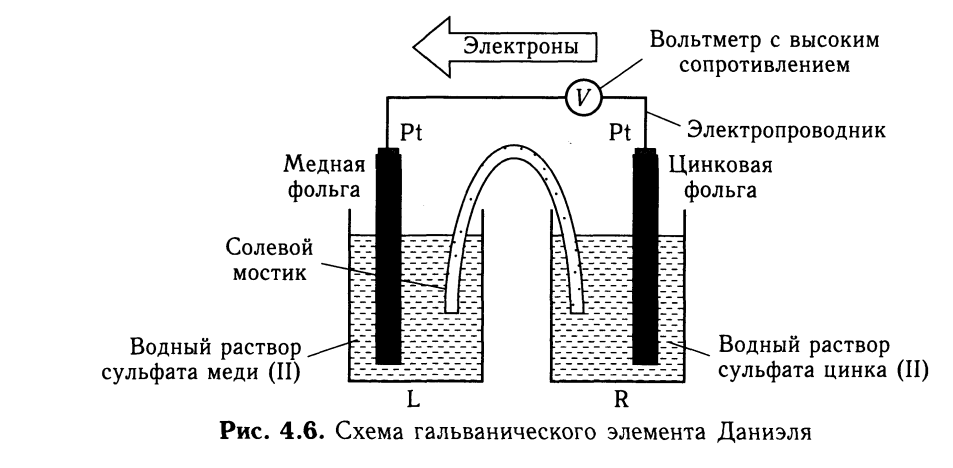
\includegraphics[scale = 0.45]{201}
	\end{figure}
 	Он содержит две сопряженные окислительно-восстановительные пары 
 	\begin{align*}
 	\begin{array}{ll}
 	\mathrm{Zn}^{2+}+2 \mathrm{e} \rightarrow \mathrm{Zn}, & E_{\mathrm{Zn}^{2+} / \mathrm{Zn}}^{\circ}=-0,760 \mathrm{B} \\
 	\mathrm{Cu}^{2+}+2 \mathrm{e} \rightarrow \mathrm{Cu}, & E_{\mathrm{Cu}^{2+} / \mathrm{Cu}}^{\circ}=+0,337 \mathrm{B}
 	\end{array}	
 	\end{align*}
 	Здесь у меди стандартный потенциал выше, значит цинк будет восстановителем, а медь окислителем. Таким образом, цинковый электрод является анодом, медный - катодом. В процессе работы элемента цинк переходит с пластинки в раствор в виде $\mathrm{Zn}^{2+}$, а медь, напротив, осаждается из раствора на пластинку.
 	
 	Для гальванического элемента принята следующая форма записи:
 	$$
 	\mathrm{Zn}\left|\mathrm{ZnSO}_{4} \| \mathrm{CuSO}_{4}\right| \mathrm{Cu}
 	$$
 	где сплошная вертикальная линия | обозначает границу раздела между разными фазами, а двойная сплошная вертикальная линия || - солевой мостик (концентрированный раствор средней соли $-\mathrm{KCl}, \mathrm{KNO}_{3}, \mathrm{NH}_{4} \mathrm{NO}_{3}$ ). Солевой мостик необходим для уменьшения диффузионного потенциала - дополнительной разности потенциалов, которая возникает из-за разной скорости переноса катионов и анионов через границу раздела фаз. Гальванический элемент принято записывать так, чтобы анод находился слева.
 	
 	ЭДС такой системы очевидно равен $E = E_r - E_l$, а если в расчете на 1M действующих реагентов, то просто $E^\circ = E_r^\circ - E_l^\circ$
	
	Гальванические элементы это что-то одноразовое, развернуть реакцию нельзя. Например обычная батарейка. Напротив аккумуляторы можно заряжать. Например свинцовый 
	\begin{align*}
	\mathrm{Pb}\left|\mathrm{H}_{2} \mathrm{SO}_{4}\right| \mathrm{PbO}_{2} \mid \mathrm{Pb}
	\end{align*}
	
	Топливные элементы это те, которые работают долго за счет того, что к ним подводят топливо и уводят отработанные продукты. Типа представлены в табличке.
	\begin{figure}[H]
		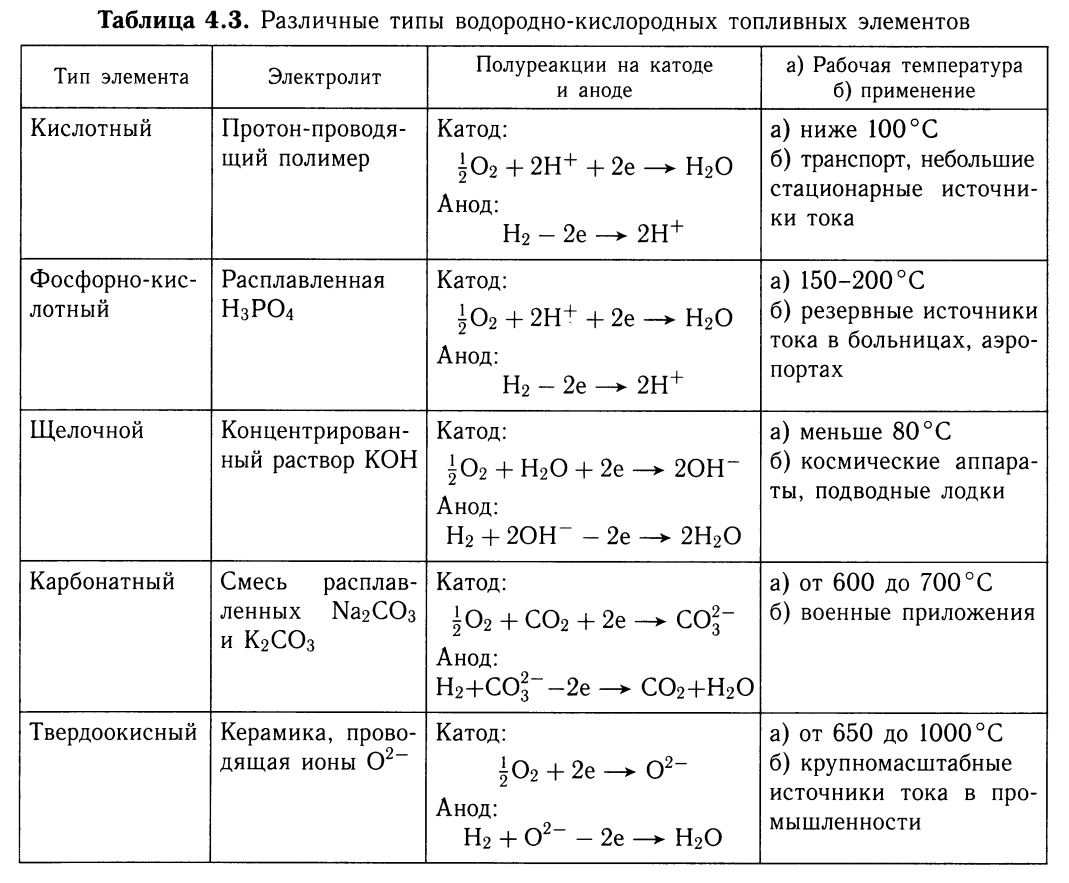
\includegraphics[width=0.7\linewidth]{202}
	\end{figure}
	\subsection{Электролиз}
	\textbf{Электролиз -- окислительно восстановительный процесс, вызванный действием постоянного тока}
	В каком-то смысле это обратный к химическому получению тока процесс. В первом случае мы выкачивали энергию из реакции в цепь, а здесь наоборот закачиваем ее. Поэтому таким образом можно провести даже те реакции, которые вроде бы запрещает термодинамика.
	
	Рассмотрим, например, электролиз расплава $\ce{NaCl}$
	На катоде натрий будет восстанавливаться до металла $\ce{Na^+ + e -> Na}$ а на аноде хлор перейдет в свободное состояние $\ce{2Cl^-  - 2e -> Cl_2}$	
	Таким образом хлорид натрия разлагается на простые вещества.
	
	Если проводить опыт не в расплаве, а в водном растворе, то все немного сложнее. Потому что вода сама может в процессе электролиза разложиться на чистые кислород и водород. Надо понять что будет реагировать первым.
	\begin{align*}
	&\ce{2H_2O + 2e -> H_2 + 2HO^-} &E^0 = - 0.828 V\\
	&\ce{Na^+ + e -> Na}  &E^0  = -2.714V
	\end{align*}
	Как видно вода слабый окислитель, но натрий еще слабее. Поэтому на катоде восстанавливаться будет кислород. На аноде напротив хлор сильнее воды, там будет он будет окисляться. Итого мы получим хлор, водород и щелочь.
	\begin{figure}[H]
		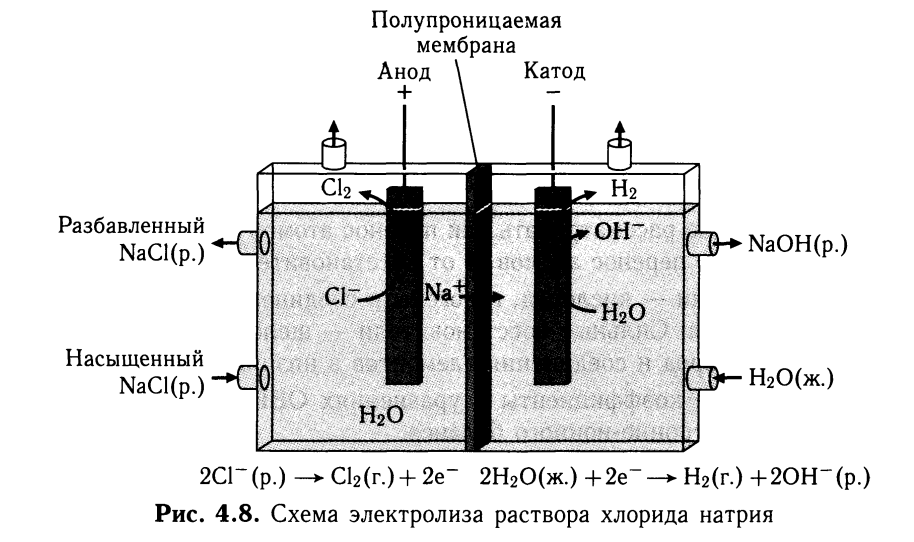
\includegraphics[scale = 0.4]{203}
	\end{figure}

\newpage

\input{TeX_Files/21.tex}

\newpage

\input{TeX_Files/22.tex}

\newpage

\input{TeX_Files/23.tex}

\newpage

\section{Подгруппа азота. Типичные степени окисления. Строение простых веществ. Водородные соединения.
Получение и свойства аммиака, соли аммония. Кислородные кислоты азота и фосфора.}
\subsection{Подгруппа азота}
\begin{wrapfigure}[24]{r}{0.2\textwidth}
\centering
\begin{tikzpicture}
\filldraw[fill=red!22!white] (-0.7,0.5) -- (-0.7,-0.5) -- (0.7,-0.5) -- (0.7,0.5) -- cycle;
\node[] at (-0.4,0.2) {\ce{N}};
\node[] at (0.4,0.2) {7};
\node[] at (0.0, -0.25) {\tiny Азот};
\filldraw[fill=red!22!white,yshift=-1.1cm] (-0.7,0.5) -- (-0.7,-0.5) -- (0.7,-0.5) -- (0.7,0.5) -- cycle;
\node[yshift=-1.1cm] at (-0.4,0.2) {\ce{P}};
\node[yshift=-1.1cm] at (0.4,0.2) {15};
\node[yshift=-1.1cm] at (0.0, -0.25) {\tiny Фосфор};
\filldraw[fill=yellow!22!white,yshift=-2.2cm] (-0.7,0.5) -- (-0.7,-0.5) -- (0.7,-0.5) -- (0.7,0.5) -- cycle;
\node[yshift=-2.2cm] at (-0.4,0.2) {\ce{As}};
\node[yshift=-2.2cm] at (0.4,0.2) {33};
\node[yshift=-2.2cm] at (0.0, -0.25) {\tiny Мышьяк};
\filldraw[fill=yellow!22!white,yshift=-3.3cm] (-0.7,0.5) -- (-0.7,-0.5) -- (0.7,-0.5) -- (0.7,0.5) -- cycle;
\node[yshift=-3.3cm] at (-0.4,0.2) {\ce{Sb}};
\node[yshift=-3.3cm] at (0.4,0.2) {51};
\node[yshift=-3.3cm] at (0.0, -0.25) {\tiny Сурьма};
\filldraw[fill=blue!22!white,yshift=-4.4cm] (-0.7,0.5) -- (-0.7,-0.5) -- (0.7,-0.5) -- (0.7,0.5) -- cycle;
\node[yshift=-4.4cm] at (-0.4,0.2) {\ce{Bi}};
\node[yshift=-4.4cm] at (0.4,0.2) {83};
\node[yshift=-4.4cm] at (0.0, -0.25) {\tiny Висмут};
\filldraw[fill=blue!22!white,yshift=-5.5cm] (-0.7,0.5) -- (-0.7,-0.5) -- (0.7,-0.5) -- (0.7,0.5) -- cycle;
\node[yshift=-5.5cm] at (-0.4,0.2) {\ce{Mc}};
\node[yshift=-5.5cm] at (0.35,0.2) {115};
\node[yshift=-5.5cm] at (0.0, -0.25) {\tiny Московий};
\end{tikzpicture}
\caption{Подгруппа азота. Красные -- выраженные неметаллы, жёлтые -- полуметаллы, синие -- металлы.}
\label{fig:azotgruop}
\end{wrapfigure}
В подгруппу азота входят сам азот, фосфор, мышьяк, сурьма, висмут и московий (последний мало интересен с точки зрения химии, т.к. период его полураспада даже для самых стабильных ядер составляет несколько десятков милисекнд) см. рис.~\ref{fig:azotgruop}. 
\begin{itemize}
    \item[\textbf{Азот}] -- бесцветный газ, не имеющий запаха  (при нормальных условиях), безвреден, не поддерживает дыхание и горение, мало растворим в воде. Азот в форме \ce{N2} состаляет больше 70\% земной атмосферы.

    Также может быть и в жидком состоянии, при температуре кипения ($−195.8 {}^{\circ}\mathrm{C}$) -- бесцветная жидкость. При контакте с воздухом поглощает кислород.

    При температуре в $−209.86 {}^{\circ}\mathrm{C}$ азот переходит в твердое состояние в виде снега. При контакте с воздухом поглощает кислород, при этом плавится, образуя раствор кислорода в азоте.
    
    \textbf{Химически свойчтва азота}:
    В свободном состояние существует в виде молекул \ce{N2}, со структурной формулой \ce{N#N}. При нормальных условиях практически не диссоциирует. Вследствие большой прочности молекулы азота некоторые его соединения эндотермичны (многие галогениды, азиды, оксиды), то есть энтальпия их образования положительна, а соединения азота термически малоустойчивы и довольно легко разлагаются при нагревании. Именно поэтому азот на Земле находится по большей части в свободном состоянии. Ввиду своей значительной инертности азот при обычных условиях реагирует только с литием:
    \begin{equation*}
        \ce{3Li + N2 -> 2Li3N}  
    \end{equation*}
    Поулучить азот можно нагревая нитрит аммония:
    \begin{equation*}
        \ce{NH4NO3 ->[t^{\circ}] 2H2O + N2 ^} 
    \end{equation*}
    Однако при этом азот ооказывается загрязнён и требует очистки. В промышленности его обычно получают из воздуха. Азот черезвычайно важен для промышленного получения аммиака.
    \item[\textbf{Фосфор}] -- в нормальных условиях фосфор существует в несколькоих аллотропных формах:
    \begin{enumerate}
        \item \textbf{Белый фосфор} -- очень активное, высокотоксичное, твёрдое, белое вещество, напоминающее парафин. Белый фосфор имеет молекулярную кристаллическую решётку, формула молекулы белого фосфора — \ce{P4}, причём атомы расположены в вершинах тетраэдра. Плохо растворяется в воде[6], но легкорастворим в органических растворителях.
        
        Химически белый фосфор чрезвычайно активен. Например, он медленно окисляется кислородом воздуха уже при комнатной температуре и светится (бледно-зелёное свечение). Явление такого рода свечения вследствие химических реакций окисления называется хемилюминесценцией (иногда ошибочно фосфоресценцией). При взаимодействии с кислородом белый фосфор горит даже под водой. 
        
        \item \textbf{Жёлтым фосфором} называют загрязнённый белый фосфор.
        \item \textbf{Красный фосфор} — это более термодинамически стабильная модификация элементарного фосфора, которая имеет формулу \ce{Р_{n}} и представляет собой полимер со сложной структурой. В зависимости от способа получения и степени дробления, красный фосфор имеет оттенки от пурпурно-красного до фиолетового, а в литом состоянии — тёмно-фиолетовый с медным оттенком, имеет металлический блеск. Химическая активность красного фосфора значительно ниже, чем у белого; ему присуща исключительно малая растворимость. Растворить красный фосфор возможно лишь в некоторых расплавленных металлах (свинец и висмут), чем иногда пользуются для получения крупных его кристаллов. Не самовоспламеняется и не люменисцирует. Красный фосфор не ядовит, используется при изготовлении тёрок спичечных коробков.
        \item \textbf{Чёрный фосфор} -- то наиболее стабильная термодинамически и химически наименее активная форма элементарного фосфора. Впервые чёрный фосфор был получен в 1914 году американским физиком П. У. Бриджменом из белого фосфора в виде чёрных блестящих кристаллов, имеющих высокую ($2690 \text{кг}/\text{м}^{3}$) плотность. Для проведения синтеза чёрного фосфора Бриджмен применил давление в $2\cdot10^{9}$ Па (20 тысяч атмосфер) и температуру около $200 {}^{\circ}\mathrm{С}$. Начало быстрого перехода лежит в области 13 000 атмосфер и температуре около $230 {}^{\circ}\mathrm{С}$.

        Чёрный фосфор представляет собой чёрное вещество с металлическим блеском, жирное на ощупь и весьма похожее на графит, и с полностью отсутствующей растворимостью в воде или органических растворителях. Поджечь чёрный фосфор можно, только предварительно сильно раскалив в атмосфере чистого кислорода до $400 {}^{\circ}\mathrm{С}$. Чёрный фосфор проводит электрический ток и имеет свойства полупроводника. Температура плавления чёрного фосфора $1000 {}^{\circ}\mathrm{С}$ под давлением $1.8\cdot10^{6}$ Па.
    \end{enumerate}
    \textbf{Химические свойства фосфора}: Легко реагирует с кислородом:
    \begin{gather*}
        \ce{4P + 5O2 -> 2P2O5} \ \text{(с избытком кислорода)}\\
        \ce{4P + 3O2 -> 2P2O3} \ \text{(с недостатком кислорода)}
    \end{gather*}
    С металлами — окислитель, образует фосфиды:
    \begin{equation*}
        \ce{2P + 3Ca -> Ca3P2}
    \end{equation*}
    C неметаллами — восстановитель:
    \begin{equation*}
        \ce{2P + 5Cl2 -> 2PCl5}
    \end{equation*}
    Фосфиды разлагаются водой и кислотами с образованием фосфина (газа аналогичного аммиаку -- \ce{PH3}).
    Сильные окислители превращают фосфор в фосфорную кислоту:
    \begin{equation*}
        \ce{2P + 5H2SO4 -> 2H3PO4 + 5SO2 + 2H2O}
    \end{equation*}
    \item[\textbf{Мышьяк}] -- как простое вещество представляет собой хрупкий полуметалл стального цвета с зеленоватым оттенком (в серой аллотропной модификации). Яд и канцероген.
    \item[\textbf{Сурьма}] --   Простое вещество сурьма — полуметалл серебристо-белого цвета с синеватым оттенком, грубозернистого строения. Известны четыре металлических аллотропных модификаций сурьмы, существующих при различных давлениях, и три аморфные модификации (взрывчатая, чёрная и жёлтая сурьма).
    \item[\textbf{Висмут}] -- Простое вещество представляет собой при нормальных условиях блестящий серебристый с розоватым оттенком металл.
    \end{itemize}
     Элементы главной подгруппы V группы имеют пять электронов на внешнем электронном уровне. В целом характеризуются как неметаллы. Способность к присоединению электронов выражена значительно слабее, по сравнению с халькогенами и галогенами. Все элементы подгруппы азота имеют электронную конфигурацию внешнего энергетического уровня атома $n\mathrm{s}^{2}n\mathrm{p}^{3}$ и могут проявлять в соединениях степени окисления от $−3$ до $+5$. Вследствие относительно меньшей электроотрицательности связь с водородом менее полярна,чем связь с водородом халькогенов и галогенов. Водородные соединения этих элементов не отщепляют в водном растворе ионы водорода, иными словами, не обладают кислотными свойствами. Первые представители подгруппы — азот и фосфор — типичные неметаллы, мышьяк и сурьма проявляют металлические свойства, висмут — типичный металл. Таким образом, в данной группе резко изменяются свойства составляющих её элементов: от типичного неметалла до типичного металла. Химия этих элементов очень разнообразна и, учитывая различия в свойствах элементов, при изучении её разбивают на две подгруппы — подгруппу азота и подгруппу мышьяка. Редко используемое альтернативное название этой группы элементов - пниктогены, в переводе с греческого языка означает удушающий, что больше относилось к первому элементу группы - азоту, который, несмотря на безвредность, не поддерживает горения и дыхания. Однако данное название в целом хорошо характеризует данную группу элементов, так как большинство из них, как в виде простого вещества, так и в виде соединений очень ядовиты.
     \subsection{Аммиак}
     \textbf{Аммиак} (нитрид водорода, аммониак, гидрид азота) — бинарное неорганическое химическое соединение азота и водорода с формулой \ce {NH3}, при нормальных условиях — бесцветный газ с резким характерным запахом.
     \subsubsection{Получение аммиака}
     В промышленности аммиак получается за счёт процесса Габера:
     \begin{equation*}
        \ce{N2 + 3H2 -> 2NH3 ^} + Q 
     \end{equation*}
     Выход аммиака зависит от условий проведения реакции, для большого выхода следует выдержать верный баланс высоких давлений и высоких температур.
     
     В лаборатории аммиак можно получать другими способами, например:
     \begin{gather*}
         \ce{NH4Cl + NaOH -> NaCl + H2O + NH3 ^}\\
         \ce{2NH4Cl + Ca(OH)2 -> CaCl2 + 2H2O + 2NH3 ^}
     \end{gather*}
     \subsubsection{Химические свойства аммиака. Аммоний. Соли аммония. Амиды.}
     Присоединяя протон аммиак образует ион аммония \ce{NH4^{+}}. Водный раствор аммиака («нашатырный спирт») имеет слабощелочную реакцию из-за протекания процесса:
     \begin{equation*}
         \ce{NH3 + H2O -> NH4^{+} + OH^{-}}
     \end{equation*}
     Взаимодействуя с кислотами, даёт соответствующие соли аммония:
    \begin{gather*}
        \ce{NH3 + HNO3 -> NH4NO3}\\
        \ce{NH3 + HCl -> NH4Cl}\\
        \ce{2NH3 + H2SO4 -> (NH4)2SO4}
    \end{gather*}
    Аммиак также способен образовывать с металлами соли — амиды, имиды и нитриды. Соединения, содержащие ионы \ce {NH2^-}, называются амидами, \ce{NH^{2-}} -- имидами, а \ce {N^{3-}} -- нитридами. Амиды щелочных металлов получают, действуя на них аммиаком:
    \begin{equation*}
        \ce{2NH3 + 2K -> 2KNH2 + H2 ^}
    \end{equation*}
    Амиды металлов являются аналогами гидроксидов. Эта аналогия усиливается тем, что ионы \ce{OH^{-}} и \ce{NH2^{-}}, а также молекулы \ce{H2O} и \ce{NH3} изоэлектронны. Амиды являются более сильными основаниями, чем гидроксиды, а следовательно, подвергаются в водных растворах необратимому гидролизу:
    \begin{equation*}
        \ce{NaNH2 + H2O -> NaOH + NH3}
    \end{equation*}
    Галогены (хлор, йод) образуют с аммиаком опасные взрывчатые вещества — галогениды азота (хлористый азот, иодистый азот).


\newpage

\section{Положение d-металлов в Периодической системе. Электронная конфигурация переходных металлов. Три ряда переходных металлов. Особенности металлов первого переходного ряда, химические свойства их соединений.}
	Переходными называют те элементы у которых частично заполнены d или f оболочки.	Переходные они потому что в таблице они находятся между p и s элементами.
	\begin{figure}[H]
		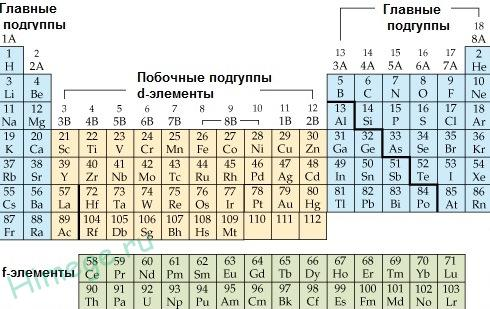
\includegraphics[scale=0.8]{252}
	\end{figure}
	Они имеют низкую энергию ионизации атома и поэтому являются металлами. В расширенной таблице они находятся посередине. Конфигурации уровней вот:
	\begin{figure}[H]
		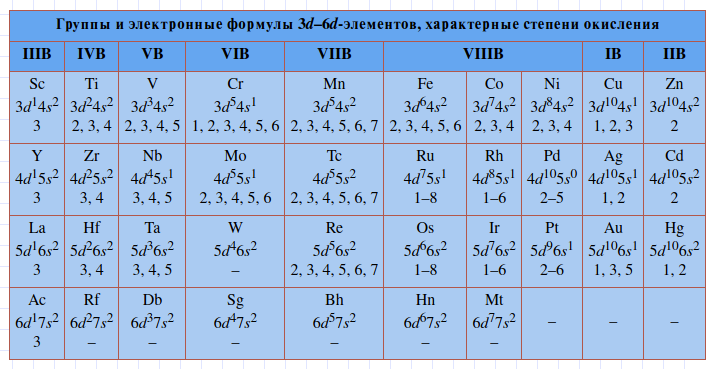
\includegraphics[scale=0.7]{251}
	\end{figure}
Иногда подгруппы называют с указанием верхнего элемента. Например подгруппа меди и тд.

Иногда VIIIB элементы первого ряда называют триадой железа, а второго и третьего платиновыми металлами. 

В каждом ряду конфигурация меняется от $(n- 1)d^1 n s^2 $ до $(n- 1)d^{10} n s^2 $ В середине и особенно конце случаются "проскоки" когда один или два электрона переходят с s уровня в d. Группа цинка особенно устойчива, потому что у нее полностью заполненный уровень. 

Перекрытие орбиталей d уровня частично объясняет прочность и тугоплавкость этих металлов. 
\subsection{Свойства 3d металлов (1 ряд)}
Все это в развернутом варианте есть в Еремине  стр 191


Все они кроме меди расположены в ряду напряжений левее водорода  и потому хорошо растворяются в кислотах 
\begin{align*}
\ce{Fe  + 2 HCl -> FeCl_2 + H_2 \uparrow}
\end{align*}
Они реагируют при нагревании с самыми активными неметаллами: кислородом и галогенами
\begin{align*}
\ce{4Cr +3O_2 -> 2 Cr_2 O_3}
\end{align*}
С менее активными неметаллами: серой, фосфором, углеродом они образуют необычные соединения
\begin{align*}
\ce{Mn + 4P -> MnP_4}
\end{align*}
Все 3d металлы получают восстановлением из оксидов водородом, углеродом или активными металлами
\begin{align*}
\ce{Ti  O_2 + 2Mg -> Ti + 2Mg O}
\end{align*}
В низших степенях окисления они проявляют свойства восстановителей, в высших окислителей
\begin{align*}
4 \mathrm{CuCl}+\mathrm{O}_{2}+4 \mathrm{HCl}=4 \mathrm{CuCl}_{2}+2 \mathrm{H}_{2} \mathrm{O} \quad\left(\mathrm{Cu}^{+1}-\mathrm{e} \rightarrow \mathrm{Cu}^{+2}\right)\\
2 \mathrm{KMnO}_{4}+10 \mathrm{KI}+8 \mathrm{H}_{2} \mathrm{SO}_{4}=2 \mathrm{MnSO}_{4}+5 \mathrm{I}_{2}+6 \mathrm{K}_{2} \mathrm{SO}_{4}+8 \mathrm{H}_{2} \mathrm{O} \\
\left(\mathrm{Mn}^{+7}+5 \mathrm{e} \rightarrow \mathrm{Mn}^{+2}\right)	
\end{align*}

\newpage

\input{TeX_Files/26.tex}

\end{document}